\chapter{Workflow}
\label{chap:workflow}

\section{Overview of Analog IC Design Flow}

Analog IC design is a meticulous process requiring extensive manual work and iterative refinement. Unlike digital design, which can be heavily automated, analog design demands close attention to the relationship between the design and the physical device models. While commercial tools have historically dominated this space, recent advancements in open-source software have made it possible to manage the essential tasks of analog IC design effectively.

\section{Open Source Analog IC Design Flow}

Figure \ref{fig:workflow_schematic} illustrates the sequential and iterative process employed in analog IC design using the open-source tools recommended by Efabless \parencite{efabless_com}. This workflow guides the design from concept to layout, highlighting the stages where iterations are necessary to refine the design and meet specifications.


\begin{figure}[ht!]
\centering
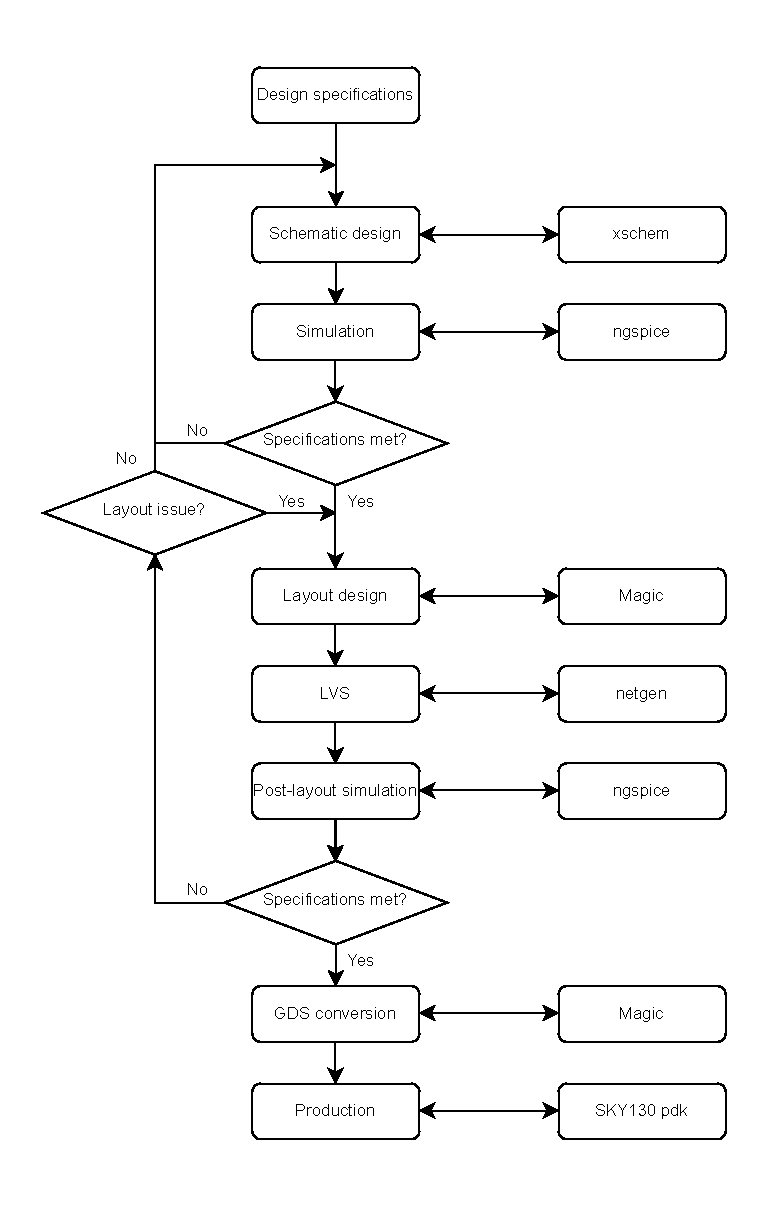
\includegraphics[width=\textwidth]{Figures/Workflow.drawio.pdf}
\caption{Analog IC Design Flow Schematic}
\label{fig:workflow_schematic}
\end{figure}


\section{Design Stages and Their Purpose}

The design stages in this workflow are as follows:

\textbf{Design Concept (Python):}
The initial stage involves formulating and modeling the idea. This stage leverages mathematical and simulation tools such as Python, along with libraries like NumPy and SciPy, to create preliminary models and validate initial concepts.

\textbf{Schematic Entry (Xschem \parencite{xschem}):}
In this stage, the design specifications are translated into a schematic diagram using tools like Xschem. Xschem simplifies the process of creating and managing schematic diagrams with its user-friendly interface.

\textbf{Simulation (ngspice) \parencite{ngspice}:}
Once the schematic is complete, the design is simulated using ngspice. This simulation tool ensures that the design operates correctly within the defined specifications, allowing for early identification and correction of any issues.

\textbf{Layout (Magic \parencite{magic}):}
The physical design stage involves drawing the geometries that will form the semiconductor device's layers. Magic is used for this purpose, providing a robust platform for creating the layout while adhering to design rules.

\textbf{Design Rule Check (DRC) (Magic):}
After the layout is complete, Magic provides an interactive DRC to validate that the layout adheres to manufacturing standards. This step is crucial for ensuring that the design can be successfully fabricated.

\textbf{Layout versus Schematic (LVS) (Netgen):}
Netgen is used to compare the LVS to ensure they match perfectly. This verification step confirms that the physical layout accurately represents the intended circuit design.

\textbf{Device and Parasitic Extraction (Magic):}
Magic also aids in the extraction of parasitic elements that occur during the layout phase. Identifying these parasitics allows for further optimization of the design, as they can impact circuit performance.

\section{Process Design Kits (PDKs)}

PDKs are vital in IC design, providing a collection of manufacturing process-specific rules, tools, and components. For this project, the SkyWater 130nm CMOS sky130 PDK \parencite{SkyWater_Technology_US_Semiconductor_Manufacturer} is utilized, offering a comprehensive suite of analog and digital design capabilities.

\section{Documentation of the Design Process in the Wiki \cite{ethz_bsse_wiki}}

Throughout this project, extensive documentation was created to aid future designers. The design process, tool presentation, installation steps, and additional resources are thoroughly detailed in the project wiki. This documentation includes:
\begin{itemize}
\item Detailed instructions on the installation and use of each tool.
\item Step-by-step guides for each stage of the design process.
\item Troubleshooting tips and best practices.
\item Links to further resources and community contributions.
\end{itemize}

For more extensive details on each tool's functions, installation, and integration with the Sky130 PDK, please refer to the wiki pages. This supplementary information provides a deeper understanding of the toolset used throughout the analog IC design process. Additionally, a small introduction to the wiki page can be found in the appendices of this report.